\section{Message Aggregation Loop Optimization for Parallel Affine Loops}\label{sec:transformation} 

This section describes modulo unrolling without unrolling (WU), our method to transform an affine loop that computes on cyclically or block-cyclically distributed data into an equivalent loop that performs message aggregation. As described in Section \ref{sec:data_distributions}, our method is not meant for block distributed data. The proposed method is based on modulo unrolling \cite{barua1999maps}, described in Section \ref{sec:modulo_unrolling}. Here we describe the method in pseudocode for simplicity and to show that this method is applicable to languages other than Chapel. 

\subsection{Modulo Unrolling Without Unrolling}\label{subsec:modulo_unrolling_without_unrolling}

Modulo unrolling increases code size because it unrolls loops by a factor equal to the number of locales (memory banks) on the system. However modulo unrolling WU for message passing machines does not increase code size. For parallel machines that use message passing, static disambiguation can be achieved by using the locale identifier without increasing the code size. Conceptually, an affine loop written in source code on a message passing machine where data is distributed cyclically among four locales such as:\newline

\tab{\texttt{\textbf{forall} i \textbf{in} 0..99 \{}}

\tab{\tab{\texttt{A[i] = B[i+2];}}}

\tab{\texttt{\}}}\newline

becomes statically disambiguated using this observation as follows:\newline

\tab{\texttt{\textbf{forall} i \textbf{in} 0..99 \textbf{by} 4 \{}}

\tab{\tab{\texttt{A[i+\$] = B[i+2+\$];}}}

\tab{\texttt{\}}}\newline

where \$ represents the locale identifier. The above is the code that is run on each locale.

\begin{figure}
	\begin{center}
	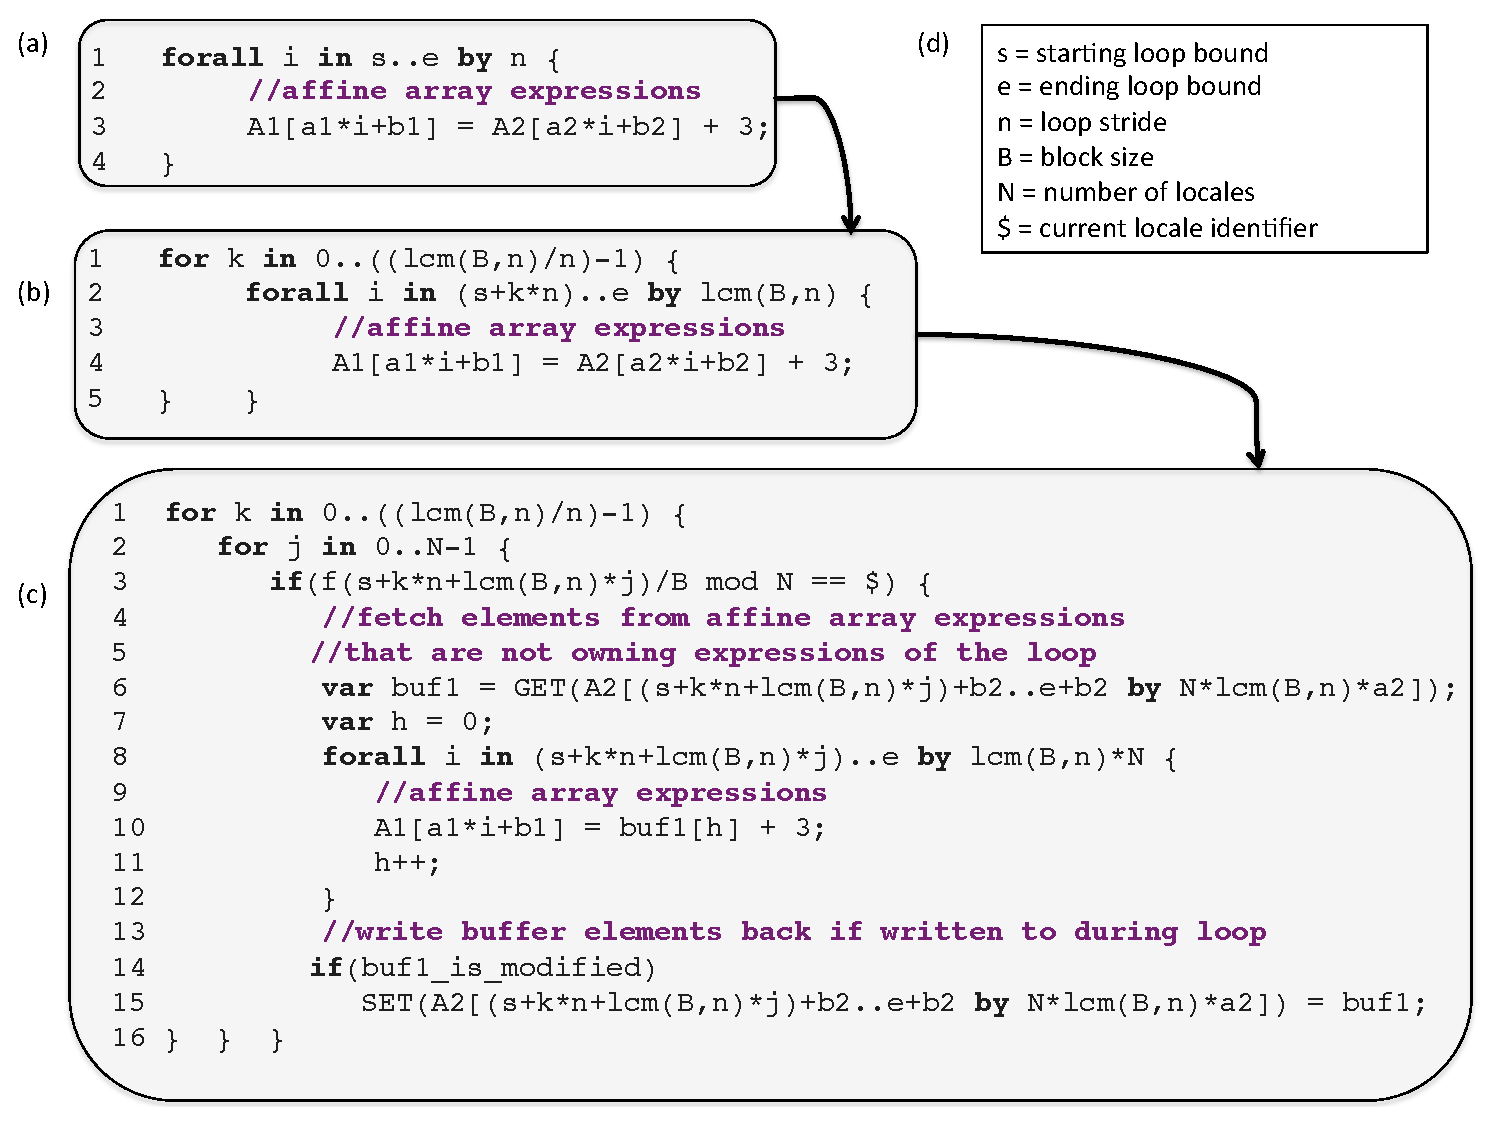
\includegraphics[scale=0.41]{./Figures/transformations}
	\caption{Steps to transform a parallel affine loop where the data is distributed cyclically or block cyclically into an equivalent loop that performs message aggregation. (a) Original parallel loop with two affine array accesses. (b) Loop after Block Cyclic transformation. After this step, the affine array accesses in loops with data distributed block cyclically will be statically disambiguated. }
	\label{transformations}
	\end{center}
\end{figure}

Figure \ref{transformations} shows how a generalized affine loop, expressed symbolically, can be transformed by our method in three steps: the Block Cyclic transformation (Figure \ref{transformations}a $\rightarrow$ Figure \ref{transformations}b), the owning expression calculation (described in Section \ref{subsec:owning_expression_calculation}), and the message aggregation (Figure \ref{transformations}b $\rightarrow$ Figure \ref{transformations}c). The optimization takes as its input a parallel \textbf{forall} loop that contains a number of affine array expressions in its loop body. Non-affine expressions are allowed in the loop body, but they are not optimized. The input loop shown in Figure \ref{transformations}a is defined by three explicit parameters: the starting loop bound $s$, the ending loop bound $e$, and the loop stride $n$. The input loop also contains two implicit parameters based on the data distribution. The number of locales the data is distributed over is $N$, and the block size, the number of consecutive array elements allocated to a single locale, is $B$. All five parameters are elements of $\mathbb{N}$. The output of the optimization is an equivalent loop structure that aggregates communication from all of the loop body's remote affine array accesses.

\subsection{Block Cyclic Transformation}\label{subsec:block_cyclic_transformation}

Modulo unrolling as described in \cite{barua1999maps} guarantees static disambiguation for data distributed cyclically but not for block-cyclically distributed data. However, we can think of a Block Cyclic distribution as $B$ adjacent Cyclic distributions, each with a cycle size that is greater than $N$. In order to achieve static disambiguation for the Block Cyclic distribution, we must transform input loops with $B >$ 1 into an equivalent loop with a loop step size that is a multiple of $B$. 

Lines 1 and 2 of Figure \ref{transformations}b show this transformation. We replace the loop step size on line 1 of Figure \ref{transformations}a with the \textit{least common multiple} of $B$ and $n$ in line 2 of Figure \ref{transformations}b. The intuition behind this new step size is that two successive loop iterations accessing the same position within a block will always be separated by a fixed stride length that is a multiple of the block size. To maintain the original meaning of the input loop, an outer \textbf{for} loop is added on line 1 of Figure \ref{transformations}b to handle iterations within each block, and the starting loop bound on line 2 is written in terms of the outer loop variable $k$. After this transformation, all affine array accesses in the loop with be statically disambiguated. This transformation is a variant of the well-known strip mining transformation which has been used for many other purposes in the literature.

The Cyclic and Block Cyclic distributions are closely related. Any Cyclic distribution can be thought of as a Block Cyclic distribution with $B$ = 1. If we apply the transformation in Figure \ref{transformations}b to a loop with cyclically distributed data, we will end up with the original input loop in Figure \ref{transformations}a, which is already statically disambiguated. 

\subsection{Owning Expression Calculation}\label{subsec:owning_expression_calculation}

There may be many affine array accesses in the input loop, each mapped to a single locale after static disambiguation. For the best communication performance, we must determine the \textit{owning expression} for the loop, which is the most common affine array expression in the loop body. More formally, the owning expression is an affine function $f(i)$, where $i$ is the loop's induction variable, that occurs statically the most number of times in the loop body. We can then use the owning expression to assign loop iterations to locales, as shown in line 3 of Figure \ref{transformations}c. 

There are two affine array accesses Figure \ref{transformations}b: $A_{1}[a_{1}i+b_{1}]$ and $A_{2}[a_{2}i+b_{2}]$. Each appears once in the loop body, so either expression can be chosen as the owning expression for the loop. For the remainder of Figure \ref{transformations}, we assume that $a_{1}i+b_{1}$ is the owning expression. 

\subsection{Message Aggregation}\label{subsec:message_aggregation}

The final step of the optimization is to aggregate all remote affine array accesses that are not accessed using the loop's owning expression before the loop starts. Figure \ref{transformations}c shows this transformation. The loop nest starting on line 2 symbolically represents which loop iterations are assigned to the $N$ locales on the system based on the owning expression calculation (line 3). In line 6, modulo unrolling WU is directly applied, as the array slice of $A_{2}$ is fetched via a single GET message and brought to a local buffer. Modulo unrolling guarantees that all elements in this array slice are remote with respect to a single locale on the loop iterations which they are used. So, they can be brought to the current locale \$ in one message. Now in lines 8-12, the affine array access $A_{2}[a_{2}i+b_{2}]$ can be replaced with an access to the local buffer. Lines 14-15 handle the case that elements brought over in bulk need to be written back to their remote locale. 

\subsection{Loops with Multi-Dimensional Array Accesses}\label{subsec:multi_dimensional}

The series of transformations described in this section and illustrated in Figure \ref{transformations} all apply to one-dimensional arrays indexed by one loop induction variable. We claim here, but do not prove, that these transformations can also be generalized to apply to certain affine array accesses for multi-dimensional arrays. The intuition for this generalization is as follows. The input affine loop now contains $m$ loop induction variables $i_{1}$, $i_{2}$, ... , $i_{m}$. Similarly, there are now $m$ starting loop bounds, ending loop bounds, loop strides, and block sizes. The $p^{th}$ block size is now the number of consecutive array elements allocated to a single locale in dimension $p$ of the array, where $1 < p < m$. Each affine array access in the loop body now contains $m$ affine array expressions where expression $p$ is an affine function of $i_{p}$. 

Under these assumptions, the transformations described in this section need only be applied to each loop induction variable independently. The owning expression calculation now produces an $m$-tuple of affine array expressions.\footnote{In our adaptation of modulo unrolling WU in Chapel, the Cyclic distribution can apply the optimization to loops with multi-dimensional array accesses, but the Block Cyclic distribution is limited to one-dimensional array accesses. This is due to the current lmitations within Chapel's Block Cyclic distribution that remained outside the scope of this work. }

 

